
\subsection{Data description}


\subsection{Estimation methodology}



\subsection{Short term abnormal returns in the Market Model}

To test hypothesis #1 and #2 of whether negative and positive SDG related events impacts firm value on the short term, I separate negative and positive events and assess the aggregated development in abnormal returns 10 days before and 10 days after an event has occurred. Moreover, I isolate the effect of the individual SDGs to test hypothesis #4 of whether events on specific sustainability goals are more relevant for investors than other. The Market Model is applied to measure abnormal returns around an event.   

\subsubsection{Negative news}

The average abnormal returns and development in cumulative average abnormal returns, inferred from the Market Model, are illustrated in figure \ref{fig:ST_neg_news}. To support the analysis, the AAR and CAAR are portrayed along with their respective 95\% confidence intervals and the amount of events on a given day relative to the event day $(t = 0)$ (right axis) illustrated by the barplot in the background. 

The left y-axis depicts the abnormal return and the x-axis is the number of days before and after an event has occurred. The average effect on returns from negative events is represented by the blue line in the graph. 
Focusing on the event date $(t=0)$ the sample average return for negative news is -0.36\%. Given the standard error of the day zero negative news AAR is  0.10\%, the z statistic is -3.45 and the null hypothesis that events has no impact is strongly rejected at a 1\% level. Hence, there is clear evidence of the news impact on day zero. The AAR on $t=1$ is equivalently negative with a value of -0.04\%, however not a significant result. The source of the day one effects is likely to be that some news are released after market closure on day zero, meaning that the effects will be captured along with the returns the day after. Moreover, the effect could be investors reacting rather slowly to news. 
More interestingly, the impact on returns is significantly negative before the identified event has taking place. 
The effect is approximately zero on average until $t = -5$ upon which the AAR decreases steadily in the days leading up to the event date. After $t=0$ the AAR surges towards neutrality at 0\% and becomes stable for the rest of the window, indicating that no short term effect is present after the event has taken place. The CAAR line shows that the market gradually learns about the prospective negative event. 
The CAAR stays negative during the full event window and bottoms on $t=2$ after a large decline of approximately $1.2\%$ from $t=-5$. 

\begin{figure} [H]
    \centering
    \caption{Negative news: AAR and CAAR}
    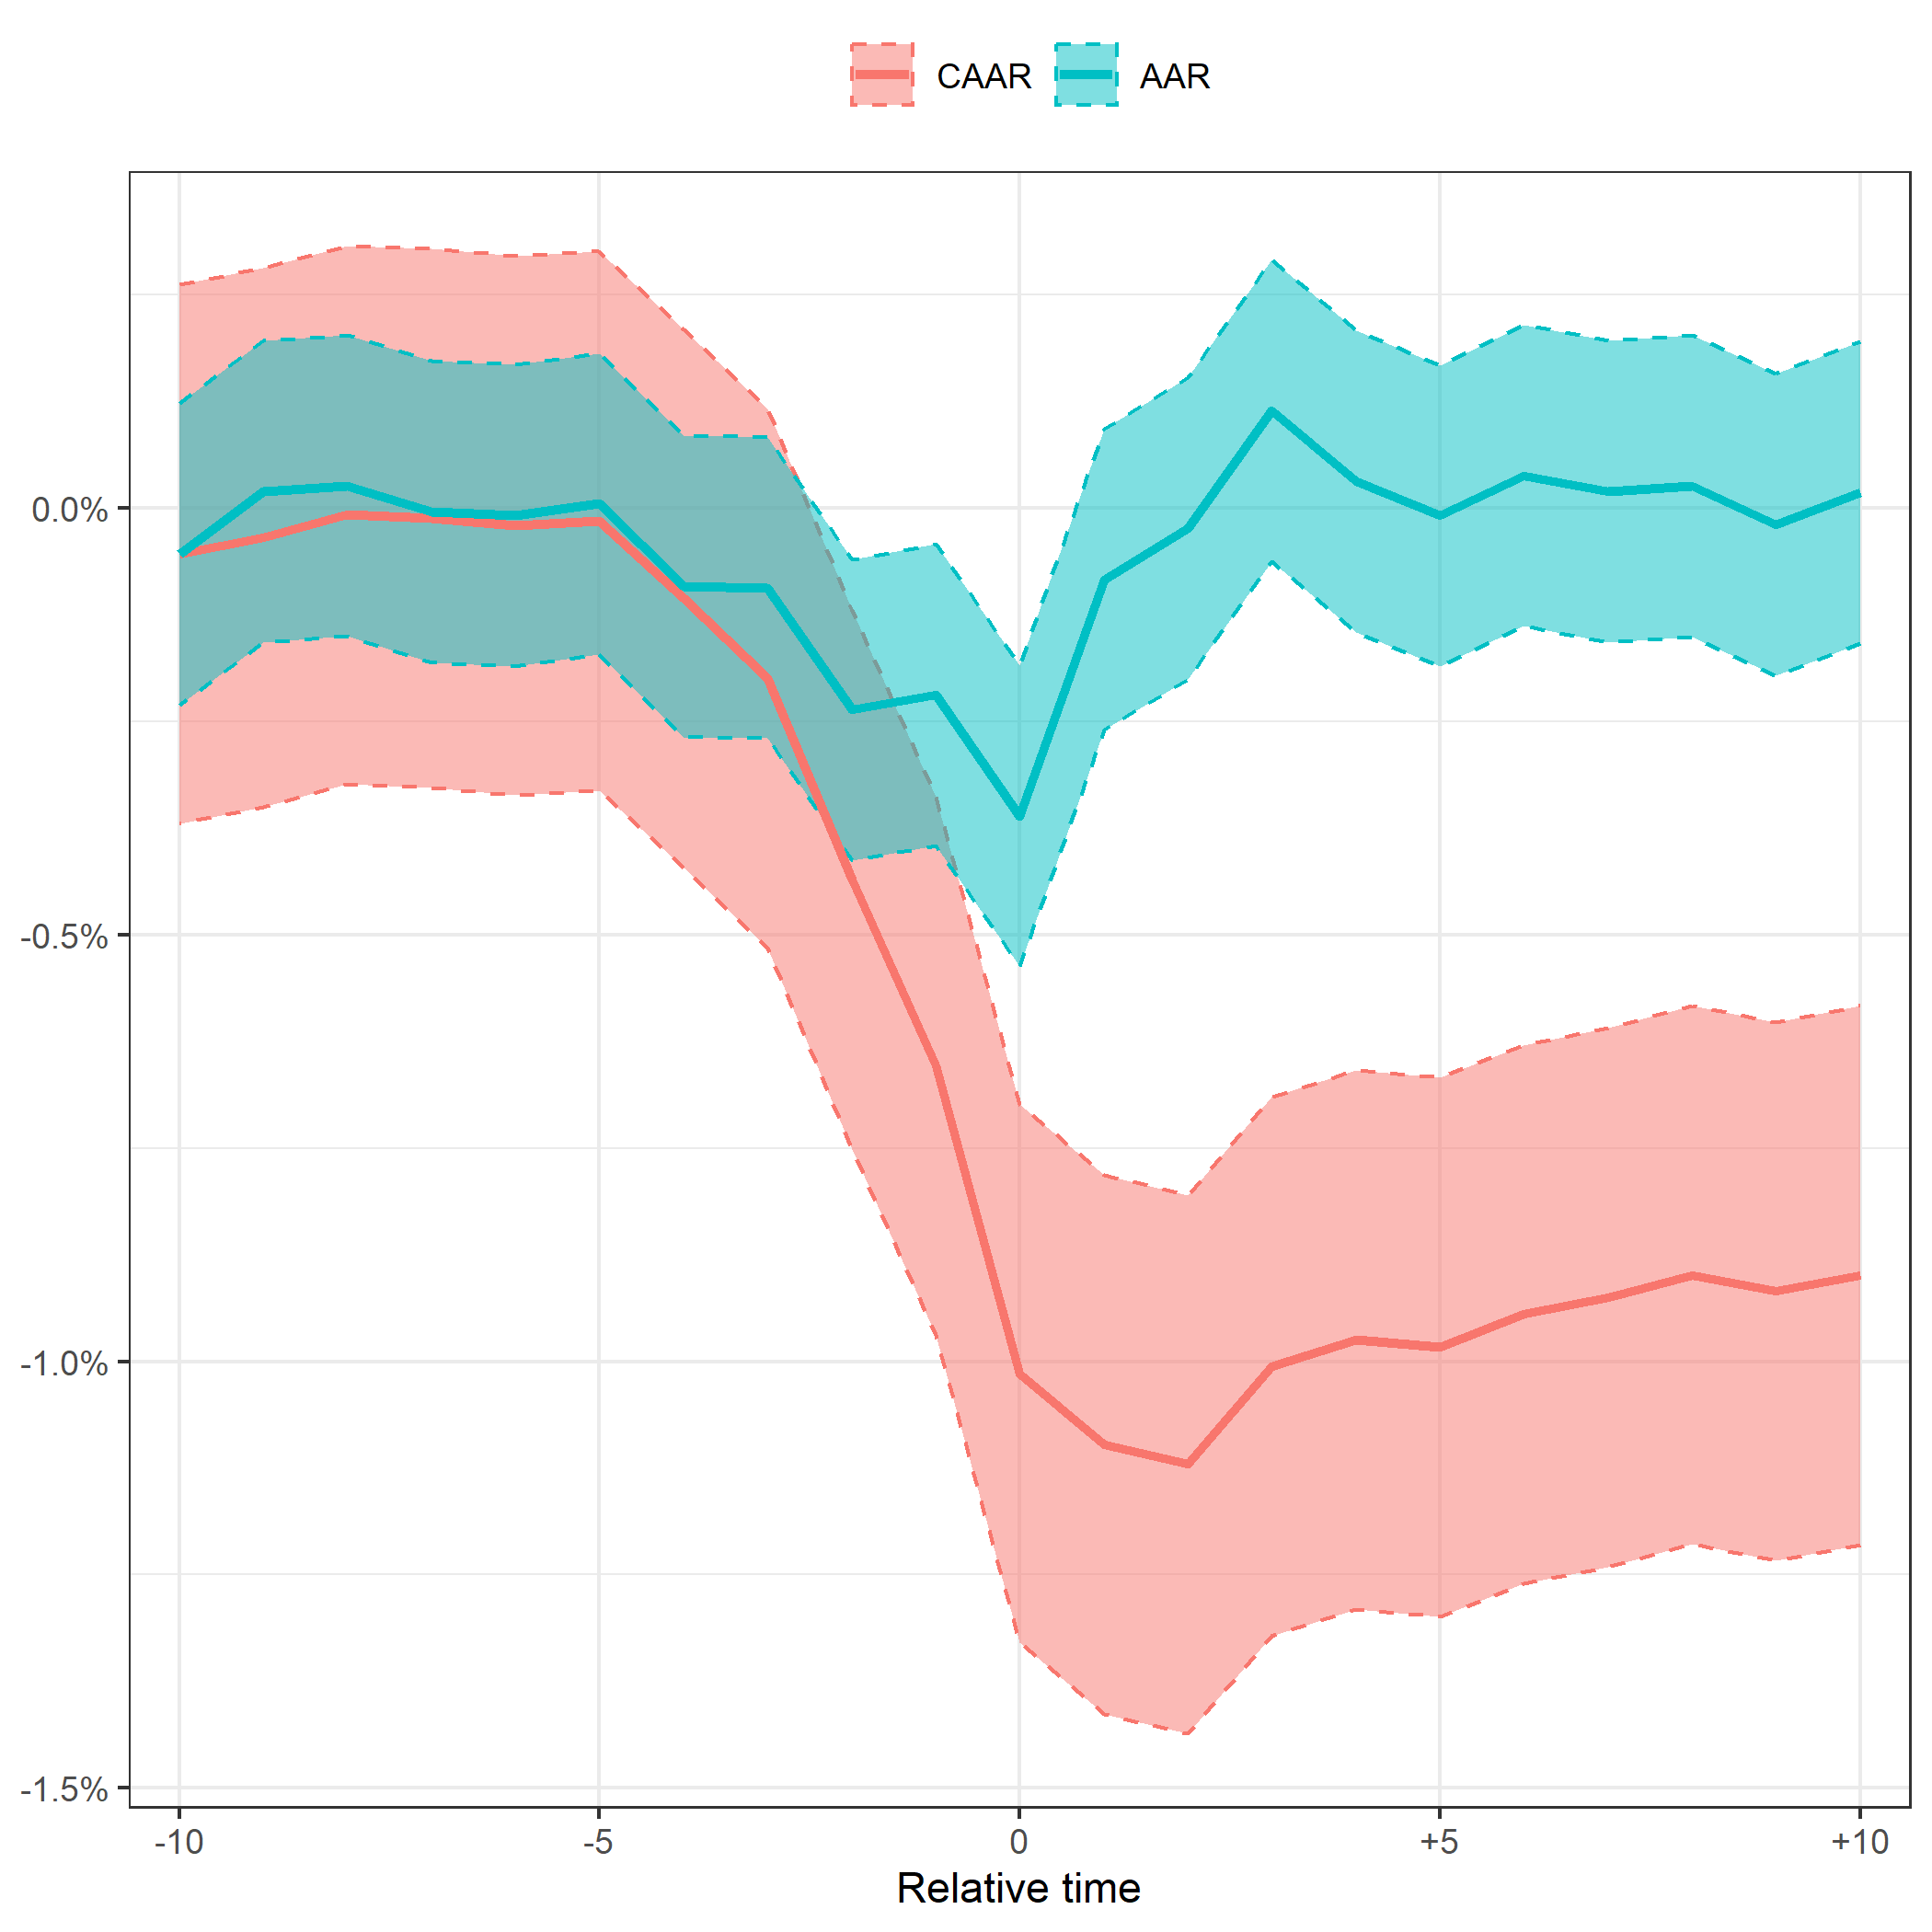
\includegraphics[scale=0.6]{Projekt/1.Figures analysis/ST_negative_all_CI.png}
     \caption*{\footnotesize The figure illustrates the average abnormal return (AAR) and cumulative AAR (CAAR) around the event date (t = 0) of negative news. The lines (left axis) represent the average and the ribbons represent the 95th confidence intervals. The bars (right axis) represent the amount of events on a given day relative to t = 0. }
    \label{fig:ST_neg_news}
\end{figure} 

However, the only significant negative AARs are found between $t=-2$ and $t=0$ at $95\%$. The same goes for the CAAR after $t=-2$ and through the remaining window. Generally, negative news seems to be priced in leading up to and including the identified event day, after which they have limited impact. \\ 
The bars offers insights into the extent of public attention leading up to an event. The bars begin to increase at $t=-5$ at which the AAR begins to decline, which imply a relation between attention towards negative news and pessimistic investor behavior even before the event date. Furthermore, this is an indication that the specified event time may be lagging the incident of the *true* event, which is a disadvantage of this model setup.  



The significance of the results in relation to negative and positive events are summarised with a z-test. The test statistic is computed and compared to its assumed distribution under the null hypothesis that the average abnormal return is zero. I use a z-test since the sample size per event day is larger than 30. The z-scores and significance complementary to the AAR on $t=0$, along with the CAAR on respectively, two, five, and 10 days around the event are presented in table \ref{tab: ST_significance}.   

The selection method for negative events was proposed to gather cases of severe negative abnormal returns. The CAAR of the full and subset windows from negative events are significantly different from zero at $p \; < 0.01$, which further validates the selection method, and that negative abnormal returns are attainable to negative events. However, the method may be late to pick up the signal of negative events or new information on the market.  

\begin{table}[ht]
\centering
\caption{AAR and CAAR over event window (in percentage)} 
\begin{tabular}{ccc}
  \hline  \hline
  & \multicolumn{1}{c}{Positive} &  \multicolumn{1}{c}{Negative}\\  
 \hline
$AAR_{t=0}$ &  $\underset{(2.123)}{0.082^{**}}$ & $\underset{(-3.509)}{-0.378^{***}}$ \\ 
$CAAR_{[-2;+2]}$  & $\underset{(0.406)}{0.032}$ & $\underset{(4.440)}{-0.715^{***}}$ \\ 
$CAAR_{[-5;+5]}$  & $\underset{(0.753)}{0.085}$ & $\underset{(-4.255)}{-0.858^{***}}$ \\ 
$CAAR_{[-10;+10]}$    & $\underset{(0.460)}{0.070}$ & $\underset{(-3.0)}{-0.822^{***}}$ \\ 
   \hline \hline
   \multicolumn{3}{p{10cm}}{ \footnotesize $^* \; p\; <\; 0.1$, $ ^{**} \; p\; <\; 0.05$, $ ^{***} \; p\; <\; 0.01$  } \\
   \multicolumn{3}{p{10cm}}{\footnotesize The tables shows the CAAR and associated t-value related to positive and negative events over an event window of 5, 10, and 21 days surrounding the event date along with the AAR on $t=0$. Positive and negative events consists of, respectively, 3564 and 1046 observations. } \\
   \hline
\end{tabular}
\label{tab: ST_significance}
\end{table}


\noindent \textbf{Split news on relation to SDGs.} Examining the average effect from, respectively, positive and negative events provides insights into the overall relational tendency between shareholder sentiment and corporate sustainability. By investigating the abnormal returns resulting from events specific to the individual SDGs one can gain a deeper understanding of which themes within corporate sustainability that investors place most emphasis with. Figure \ref{fig:ST_neg_bar} illustrates the AAR on $t=0$ from events related to specific SDGs along with corresponding confidence intervals. 

\begin{figure} [H]
    \centering
    \caption{Negative news: AAR split on relation to SDGs}
    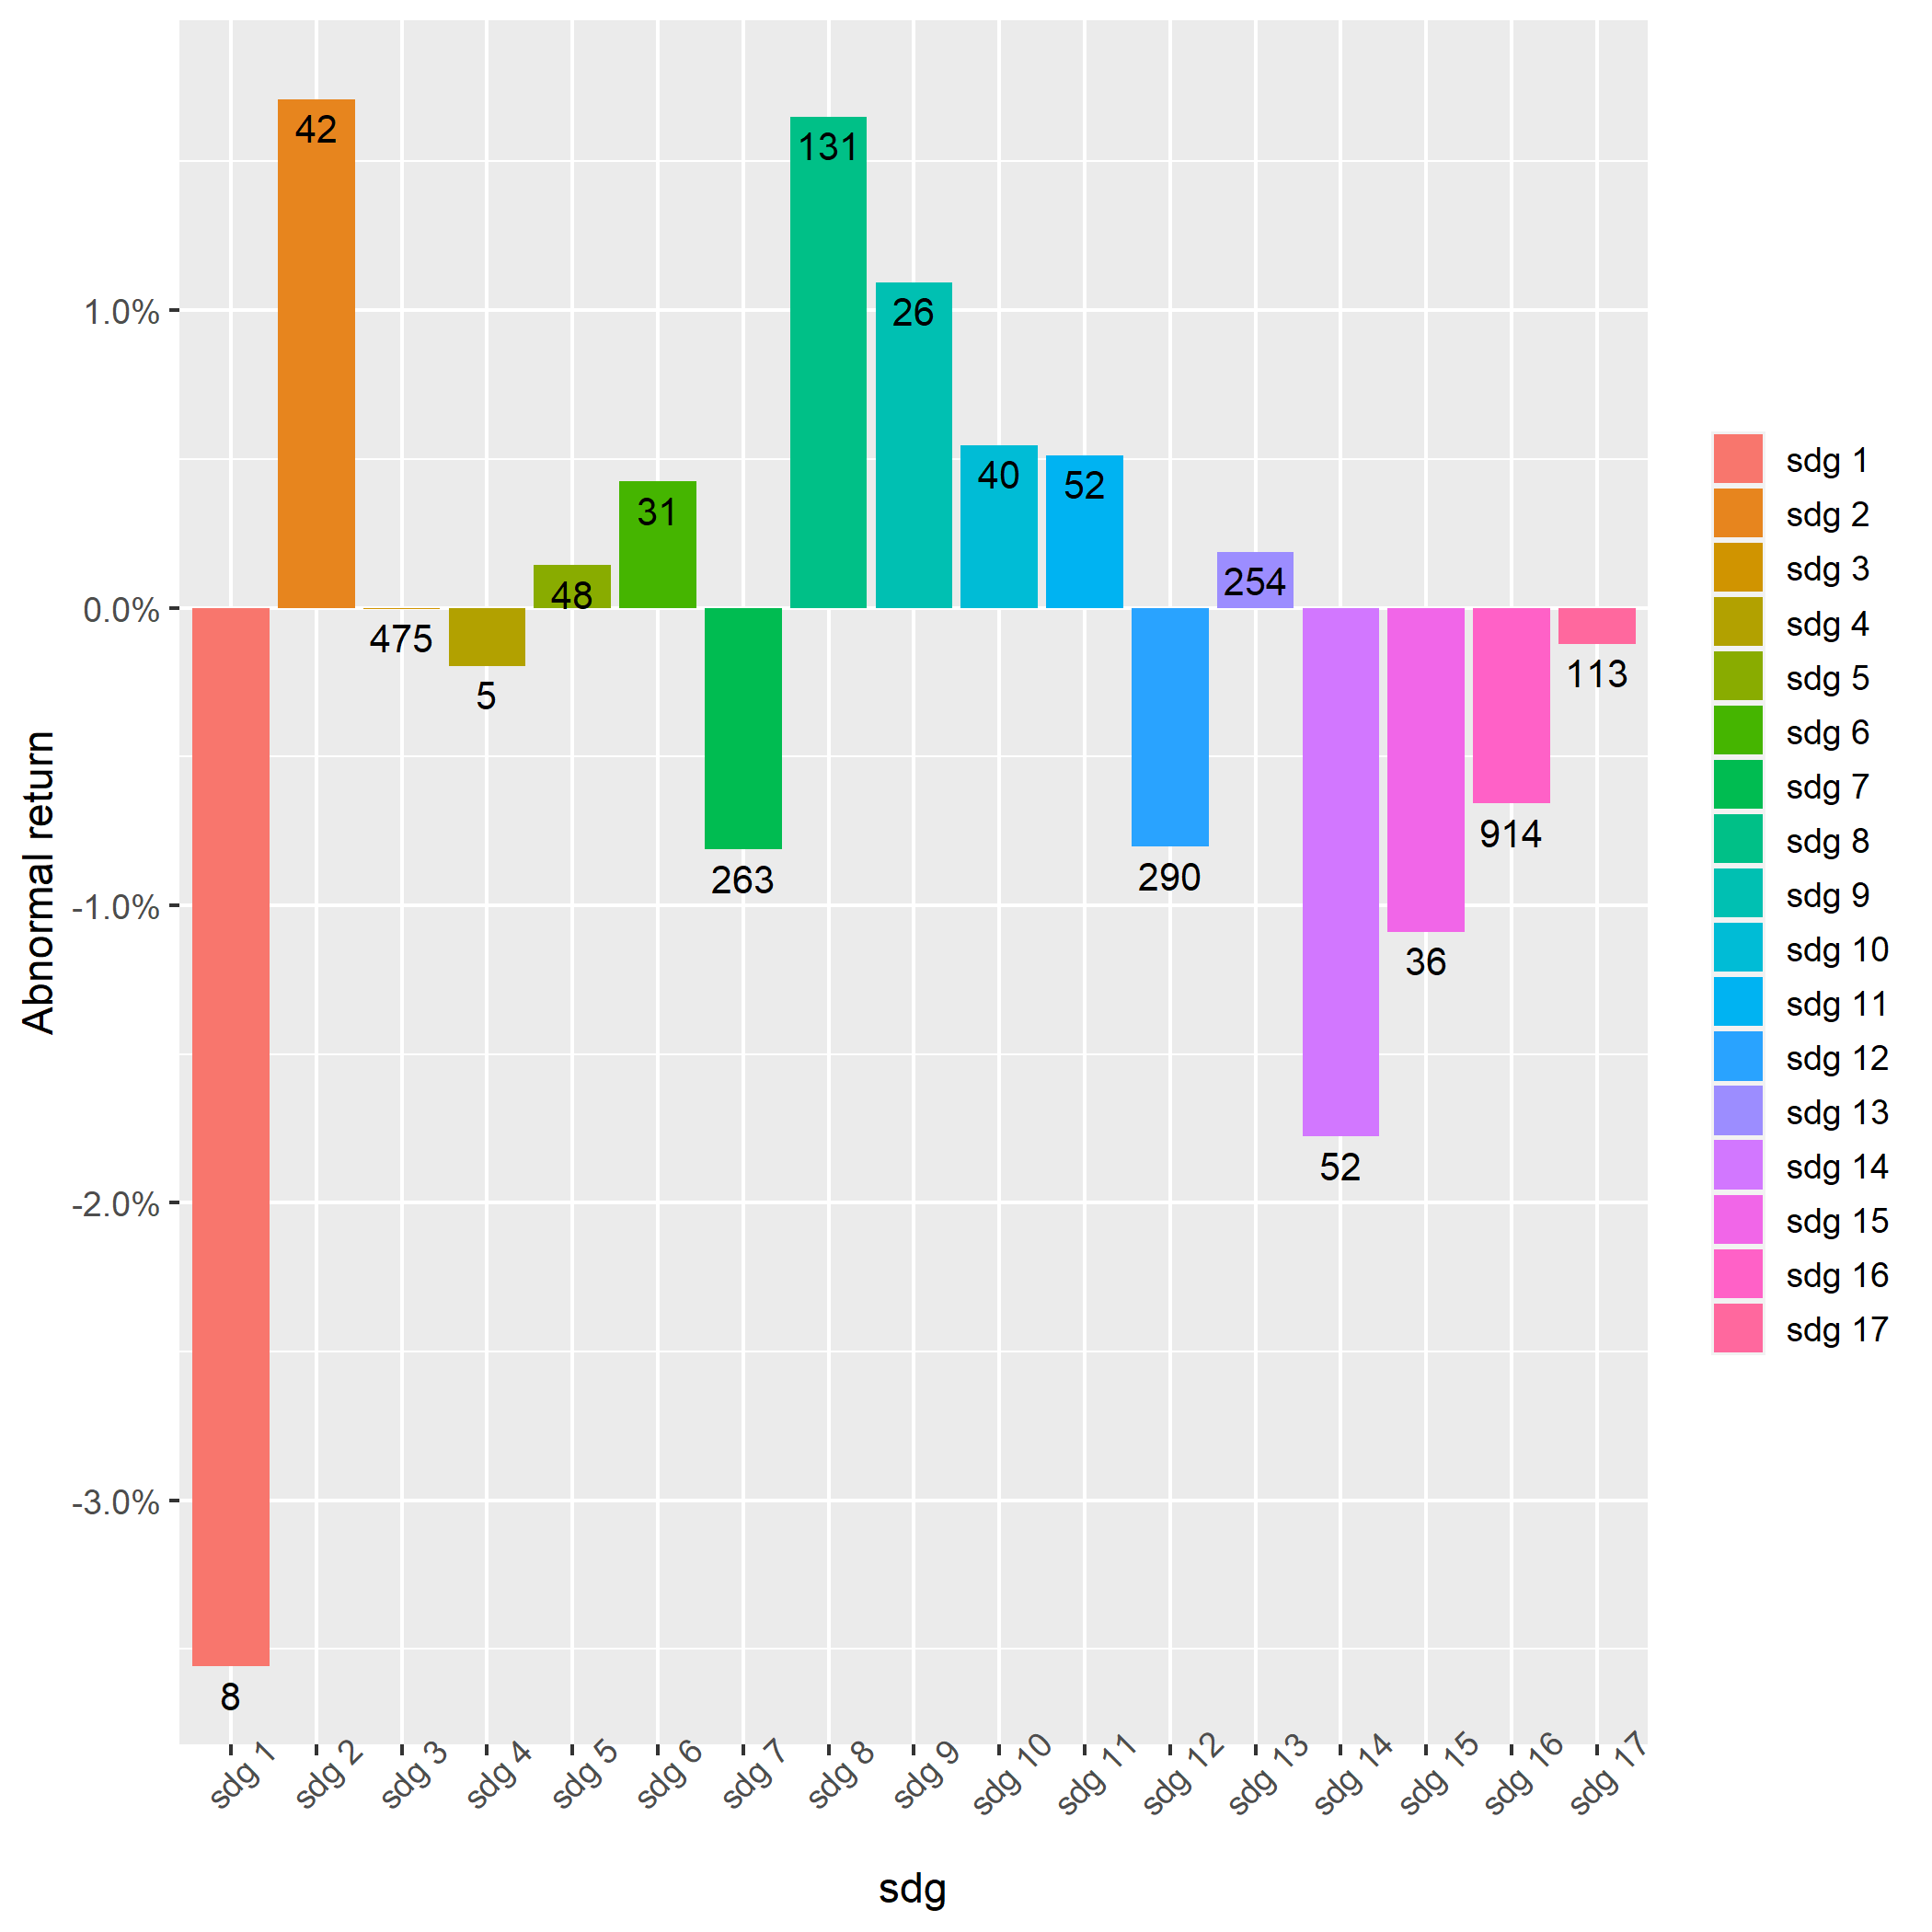
\includegraphics[scale=0.6]{Projekt/1.Figures analysis/ST_negative_sdg_bar.png}
    \caption*{\footnotesize The figure illustrates the AAR on $t = 0$ from negative news. The error bars represent the 95\% confidence intervals of the AAR.}
    \label{fig:ST_neg_bar}
\end{figure}

Splitting the events on SDGs generally illustrate that negative events in most groups are associated with negative abnormal returns. However, the statistical uncertainty in the measurements means that one cannot generate a lot of insights from the aggregated values. Only SDG 10, 16, and 17 provides abnormal returns significantly different from zero at a \% level. The statistical uncertainty originates from the relatively low amount of observations associated with the individual groups after dividing the events into SDGs. For example, SDG 4 and 9 has only, respectively, 16 and 83 observations, which results in excessively wide confidence interval, whereas SDG 12 and 16 has, respectively, 576 and 1364 observations resulting in higher statistical certainty.   

\noindent \textbf{Split firms on ESG rating.} 

The investigation of negative news and stock returns verify a significant relation between the two in the short horizon. It is of similar interest to determine whether the sustainability profile of a firm influences how investors react to news related to the social development goals. 

Figure \ref{fig:ST_neg_ESG} employs the same setup as figure \ref{fig:ST_neg_news} and includes the CAAR of an nearly identical sample\footnote{The sample is not identical as four firms were missing an ESG risk rating.} of firms and events only with a separation on the firms' ESG risk profiles. "Low" means that a firm has a low risk of encountering complications in relation to ESG affairs. Intuitively, firms with low ESG risks are expected to experience less disputes related to sustainability. Hence, if they do appear in such disputes, a logical reaction from investors would be of more severe magnitude. 

\begin{figure} [H]
    \centering
    \caption{Negative news: CAAR split on ESG rating}
    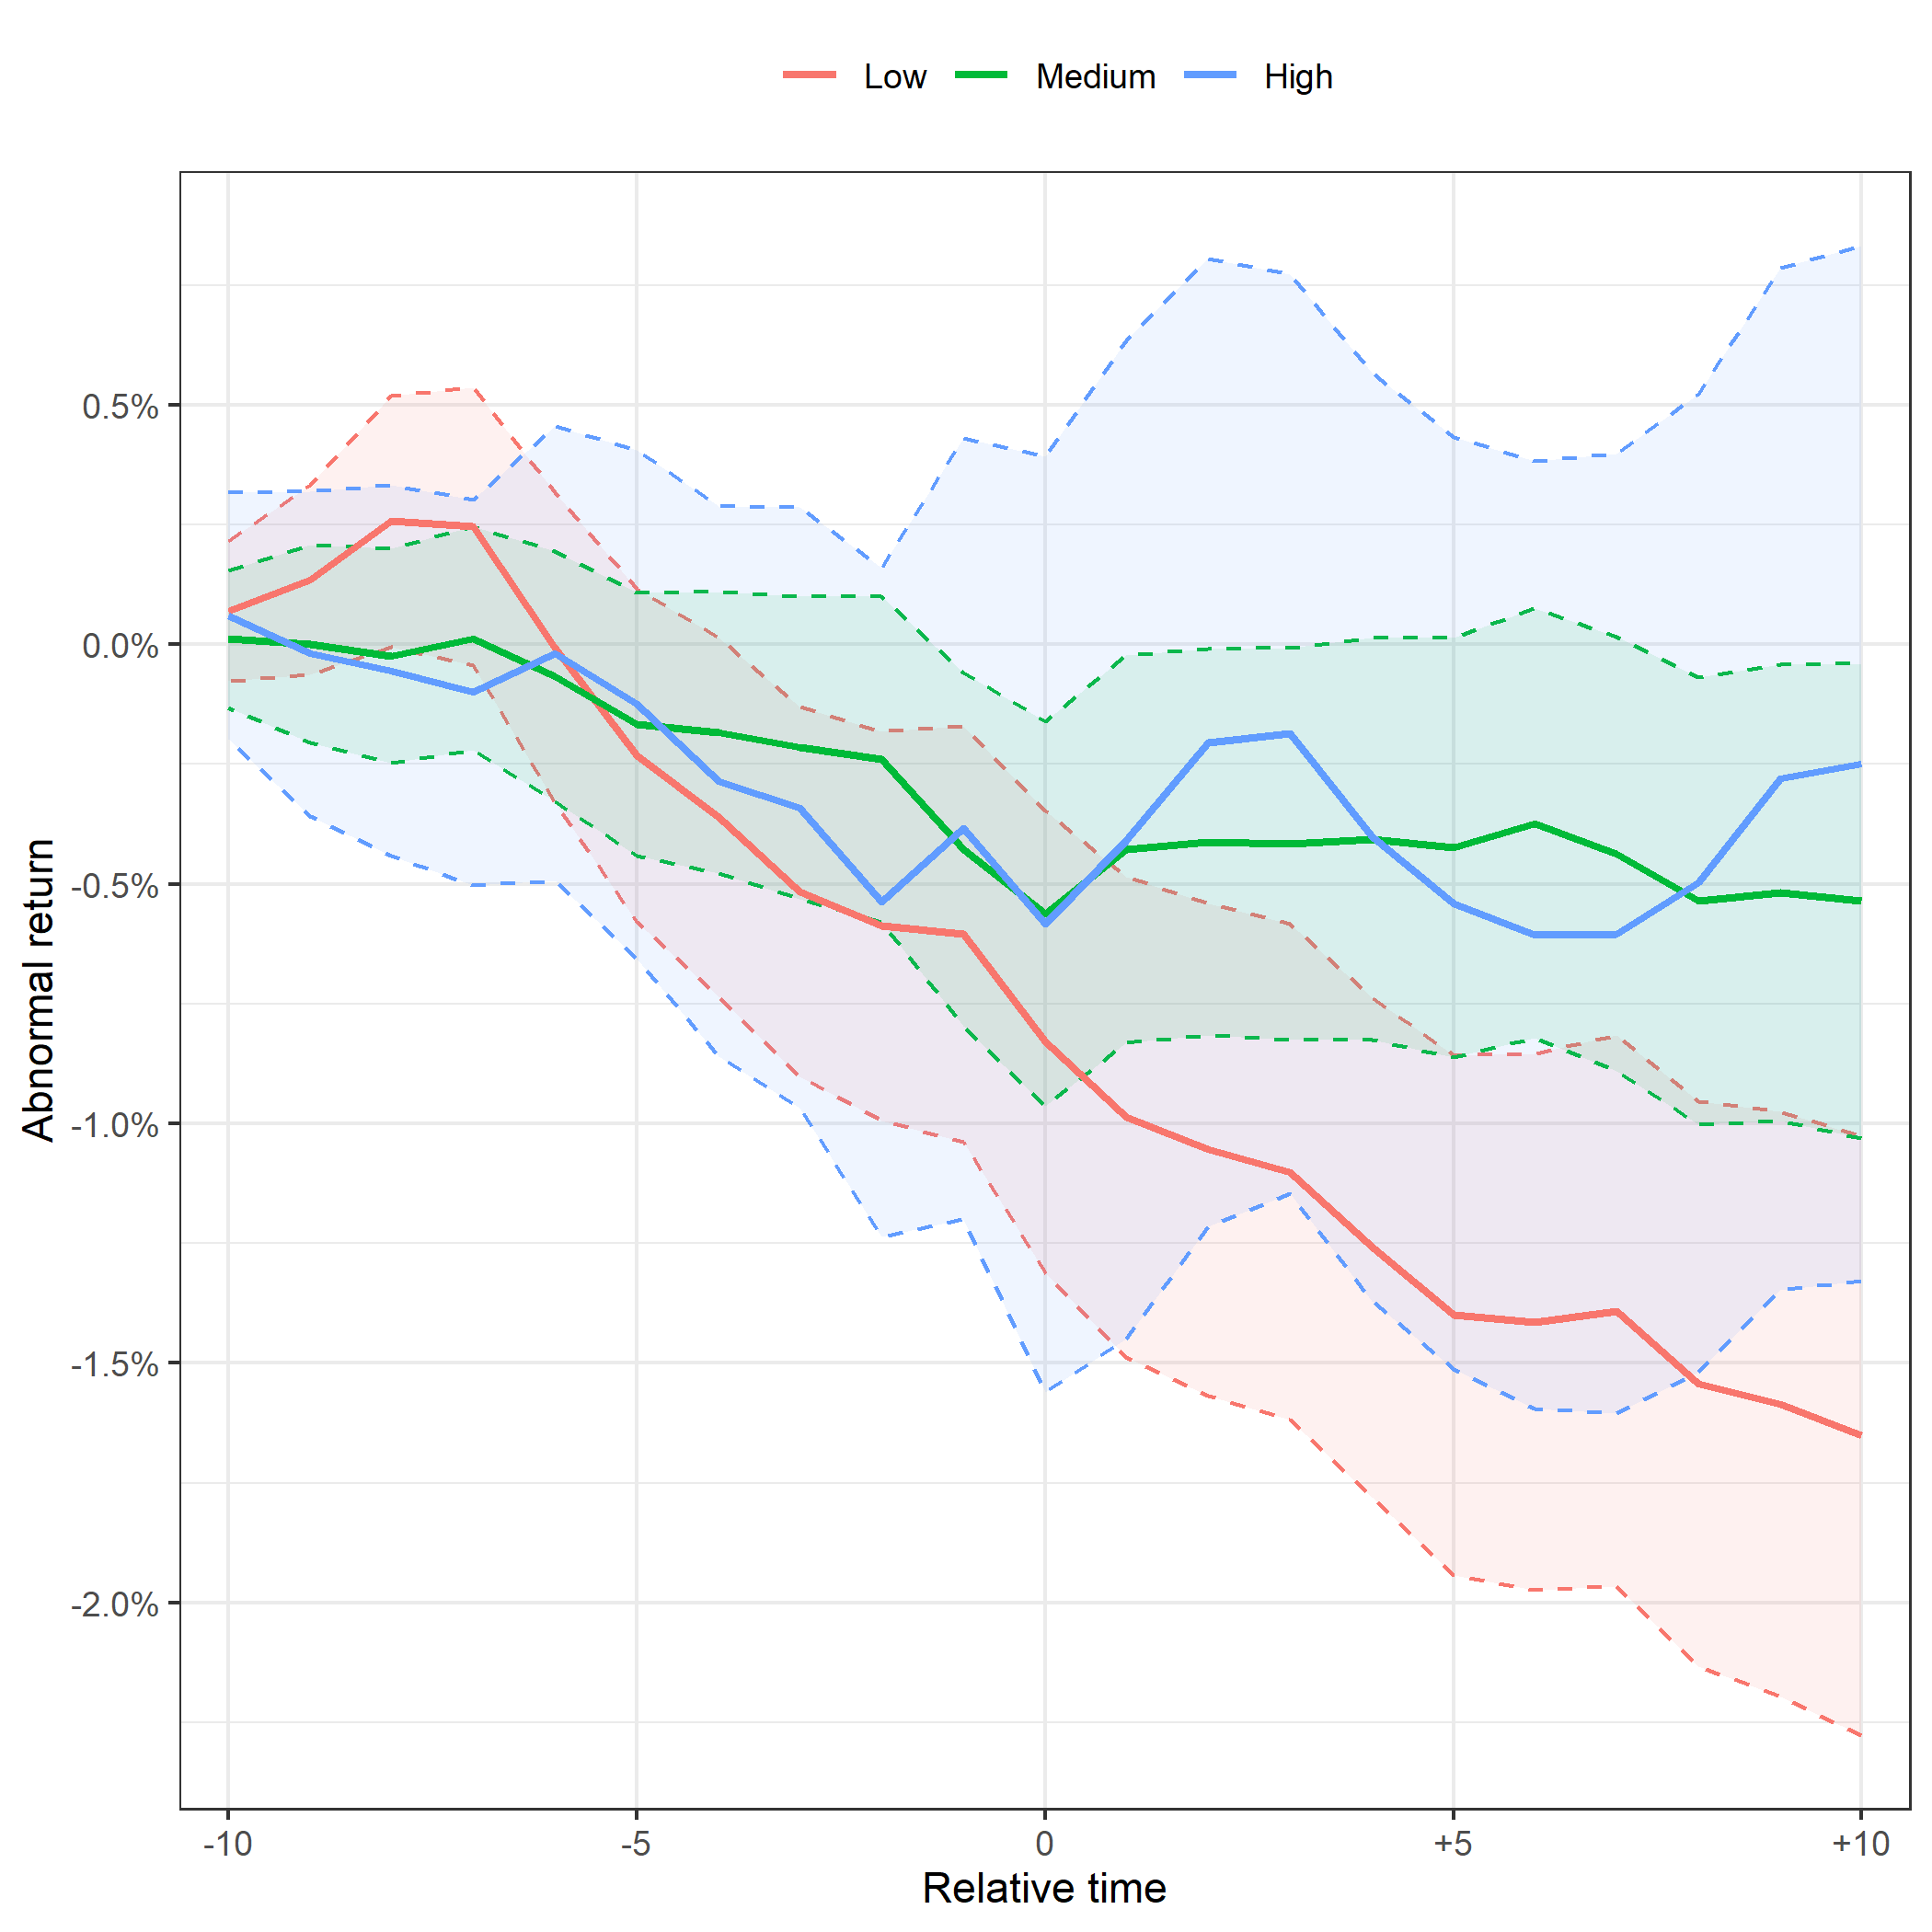
\includegraphics[scale=0.6]{Projekt/1.Figures analysis/ST_negative_ESG.png}
     \caption*{\footnotesize The figure illustrates the CAAR around the event date of negative news. The lines represent low, medium and high ESG risk of the firms in the sample. The ribbons represent the 95th confidence intervals. The categories low, medium, and high have, respectively, 315, 559, and 170 observed events in the sample. }
    \label{fig:ST_neg_ESG}
\end{figure} 


The CAAR of the three groups of risk profiles do behave in a similar way, indicating that the general pattern of a negative relation from figure \ref{fig:ST_neg_news} applies to all risk types. Nonetheless, a relation as described above do seem to occur, as firms with a low ESG risk profile are experiencing larger return declines after negative events than firms with medium or high risk. The returns of firms with a medium or high ESG risk profile appear to behave similar to each other, and neither of the CAARs are significant after the full period. Still, the CAAR of the medium risk group is significantly negative at $t=0$. As the group of high risk companies consists of only 170 observations, the confidence intervals become wide and no significant relation can be determined. Only the CAAR of the high risk group is significantly different from zero over the full event window.  

\subsubsection{Positive news}

Focusing initially on the event date, the sample average abnormal return for positive news with the market model is 0.08\%. With a standard error of 0.038\% the z value of the test is 2.12 and the null hypothesis that the event has no impact is rejected at a 5\% level. However, according to figure \ref{fig:ST_pos_news} the remaining days of the event window are not associated with significant reaction  from the shareholders. Following, the statistical uncertainty of the CAAR becomes more widespread through the event window, as indicated by the widening red ribbon. The positive tendency of the CAAR is insignificant since the measure is based on insignificant AARs, meaning that one cannot for certain state that the cumulative return is different from zero. Nonetheless, a positive reaction is inferred at $t=0$ indicating that investor do react instantly to positive news on average, however the gains seems to be depleted in the following weeks.  

\begin{figure} [H] 
    \centering
    \caption{Short term positive news: AAR and CAAR}
    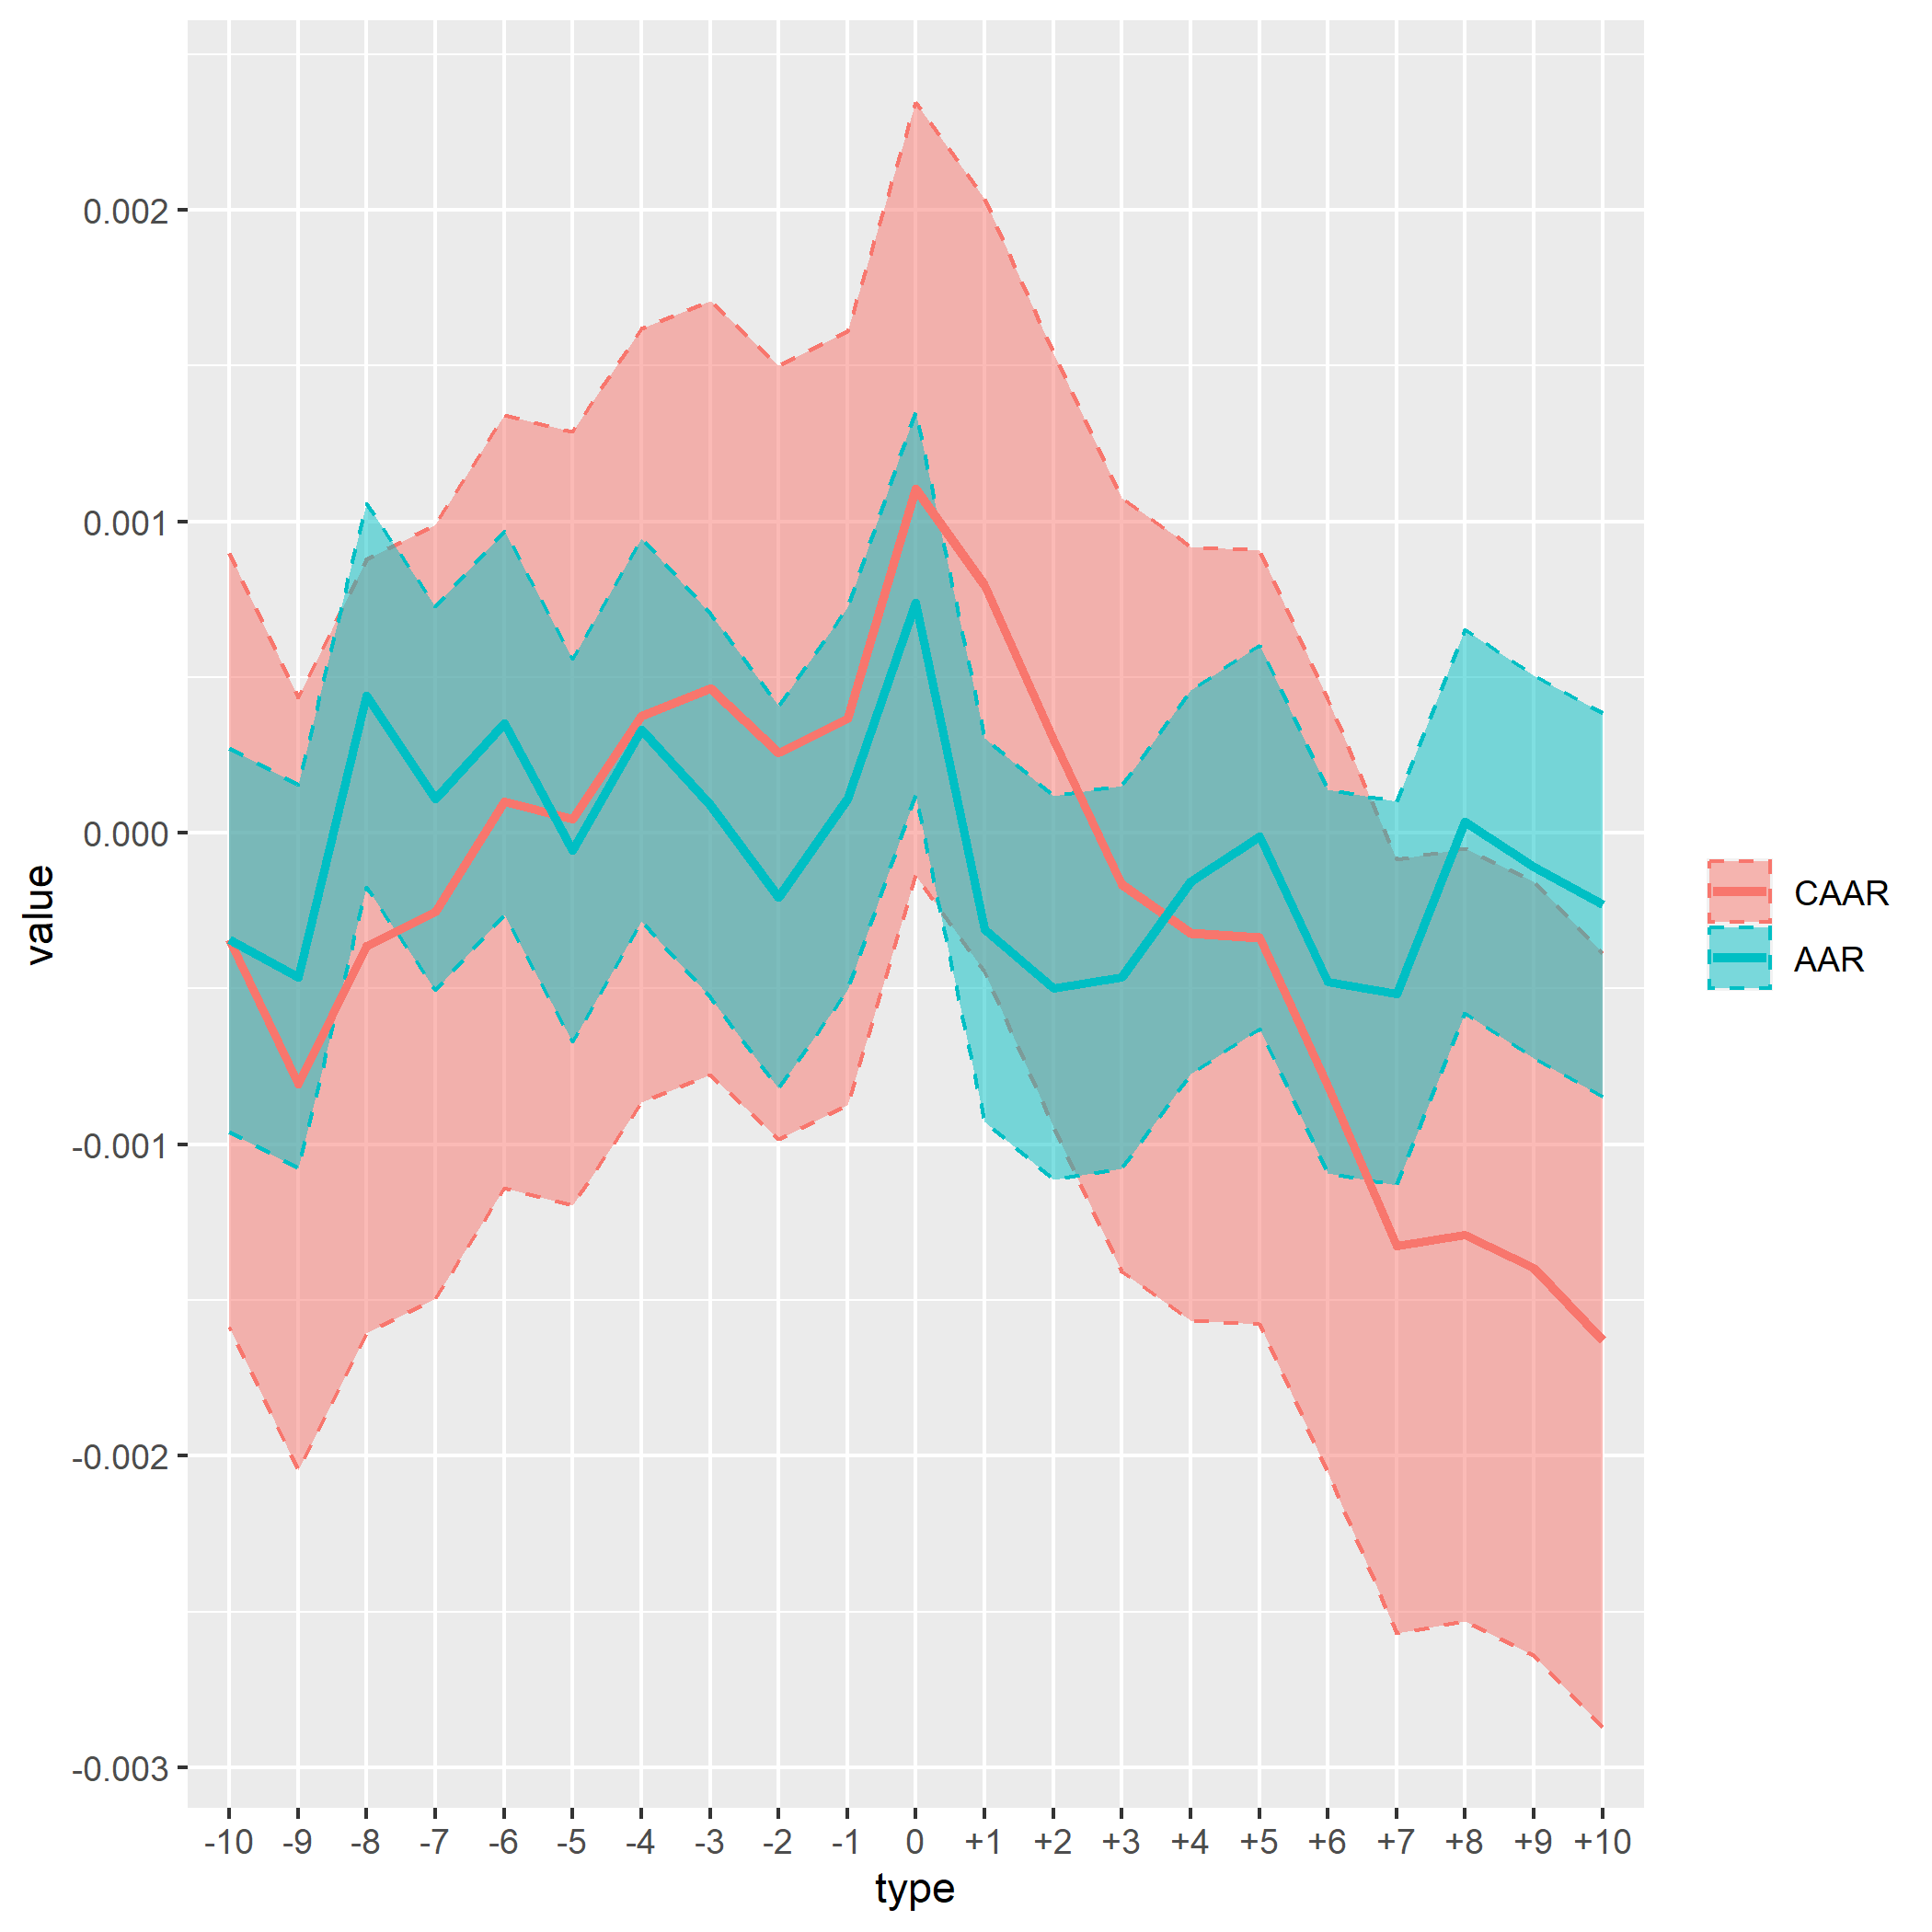
\includegraphics[scale=0.6]{Projekt/1.Figures analysis/ST_positive_all_CI.png}
    \caption*{\footnotesize The figure illustrates the average abnormal return (AAR) and cumulative AAR (CAAR) around the event date (t = 0) of positive news. The lines (left axis) represent the average and the ribbons represent the 95th confidence intervals. The bars (right axis) represent the amount of events on a given day relative to t = 0. }
    \label{fig:ST_pos_news}
\end{figure}

The insignificance of the abnormal returns associated with positive events are manifested in table \ref{tab: ST_significace}. The the CAARs on, respectively, two, five and 10 days around the event are all insignificantly different from zero. However, the AAR does exhibit positive performance at $t = 0$ at 5\% significance.


\textbf{Split news on SDGs.}
The tendency of insignificance related to positive events is further reinforced by the results from the individual SDGs, as most returns are statistically indistinguishable from zero. In contrast to the case of negative events, where the main issue was the amount of observations, the underlying issue with uncertainty comes with the seemingly random shareholder reaction to positive events, as indicated by the aggregate overview in figure \ref{fig:ST_pos_news}. Only positive news associated with SDG 7, that deals with clean energy, displays a significant, positive abnormal return. 
 
\begin{figure} [H]
    \centering
    \caption{AAR per SDG: positive news}
    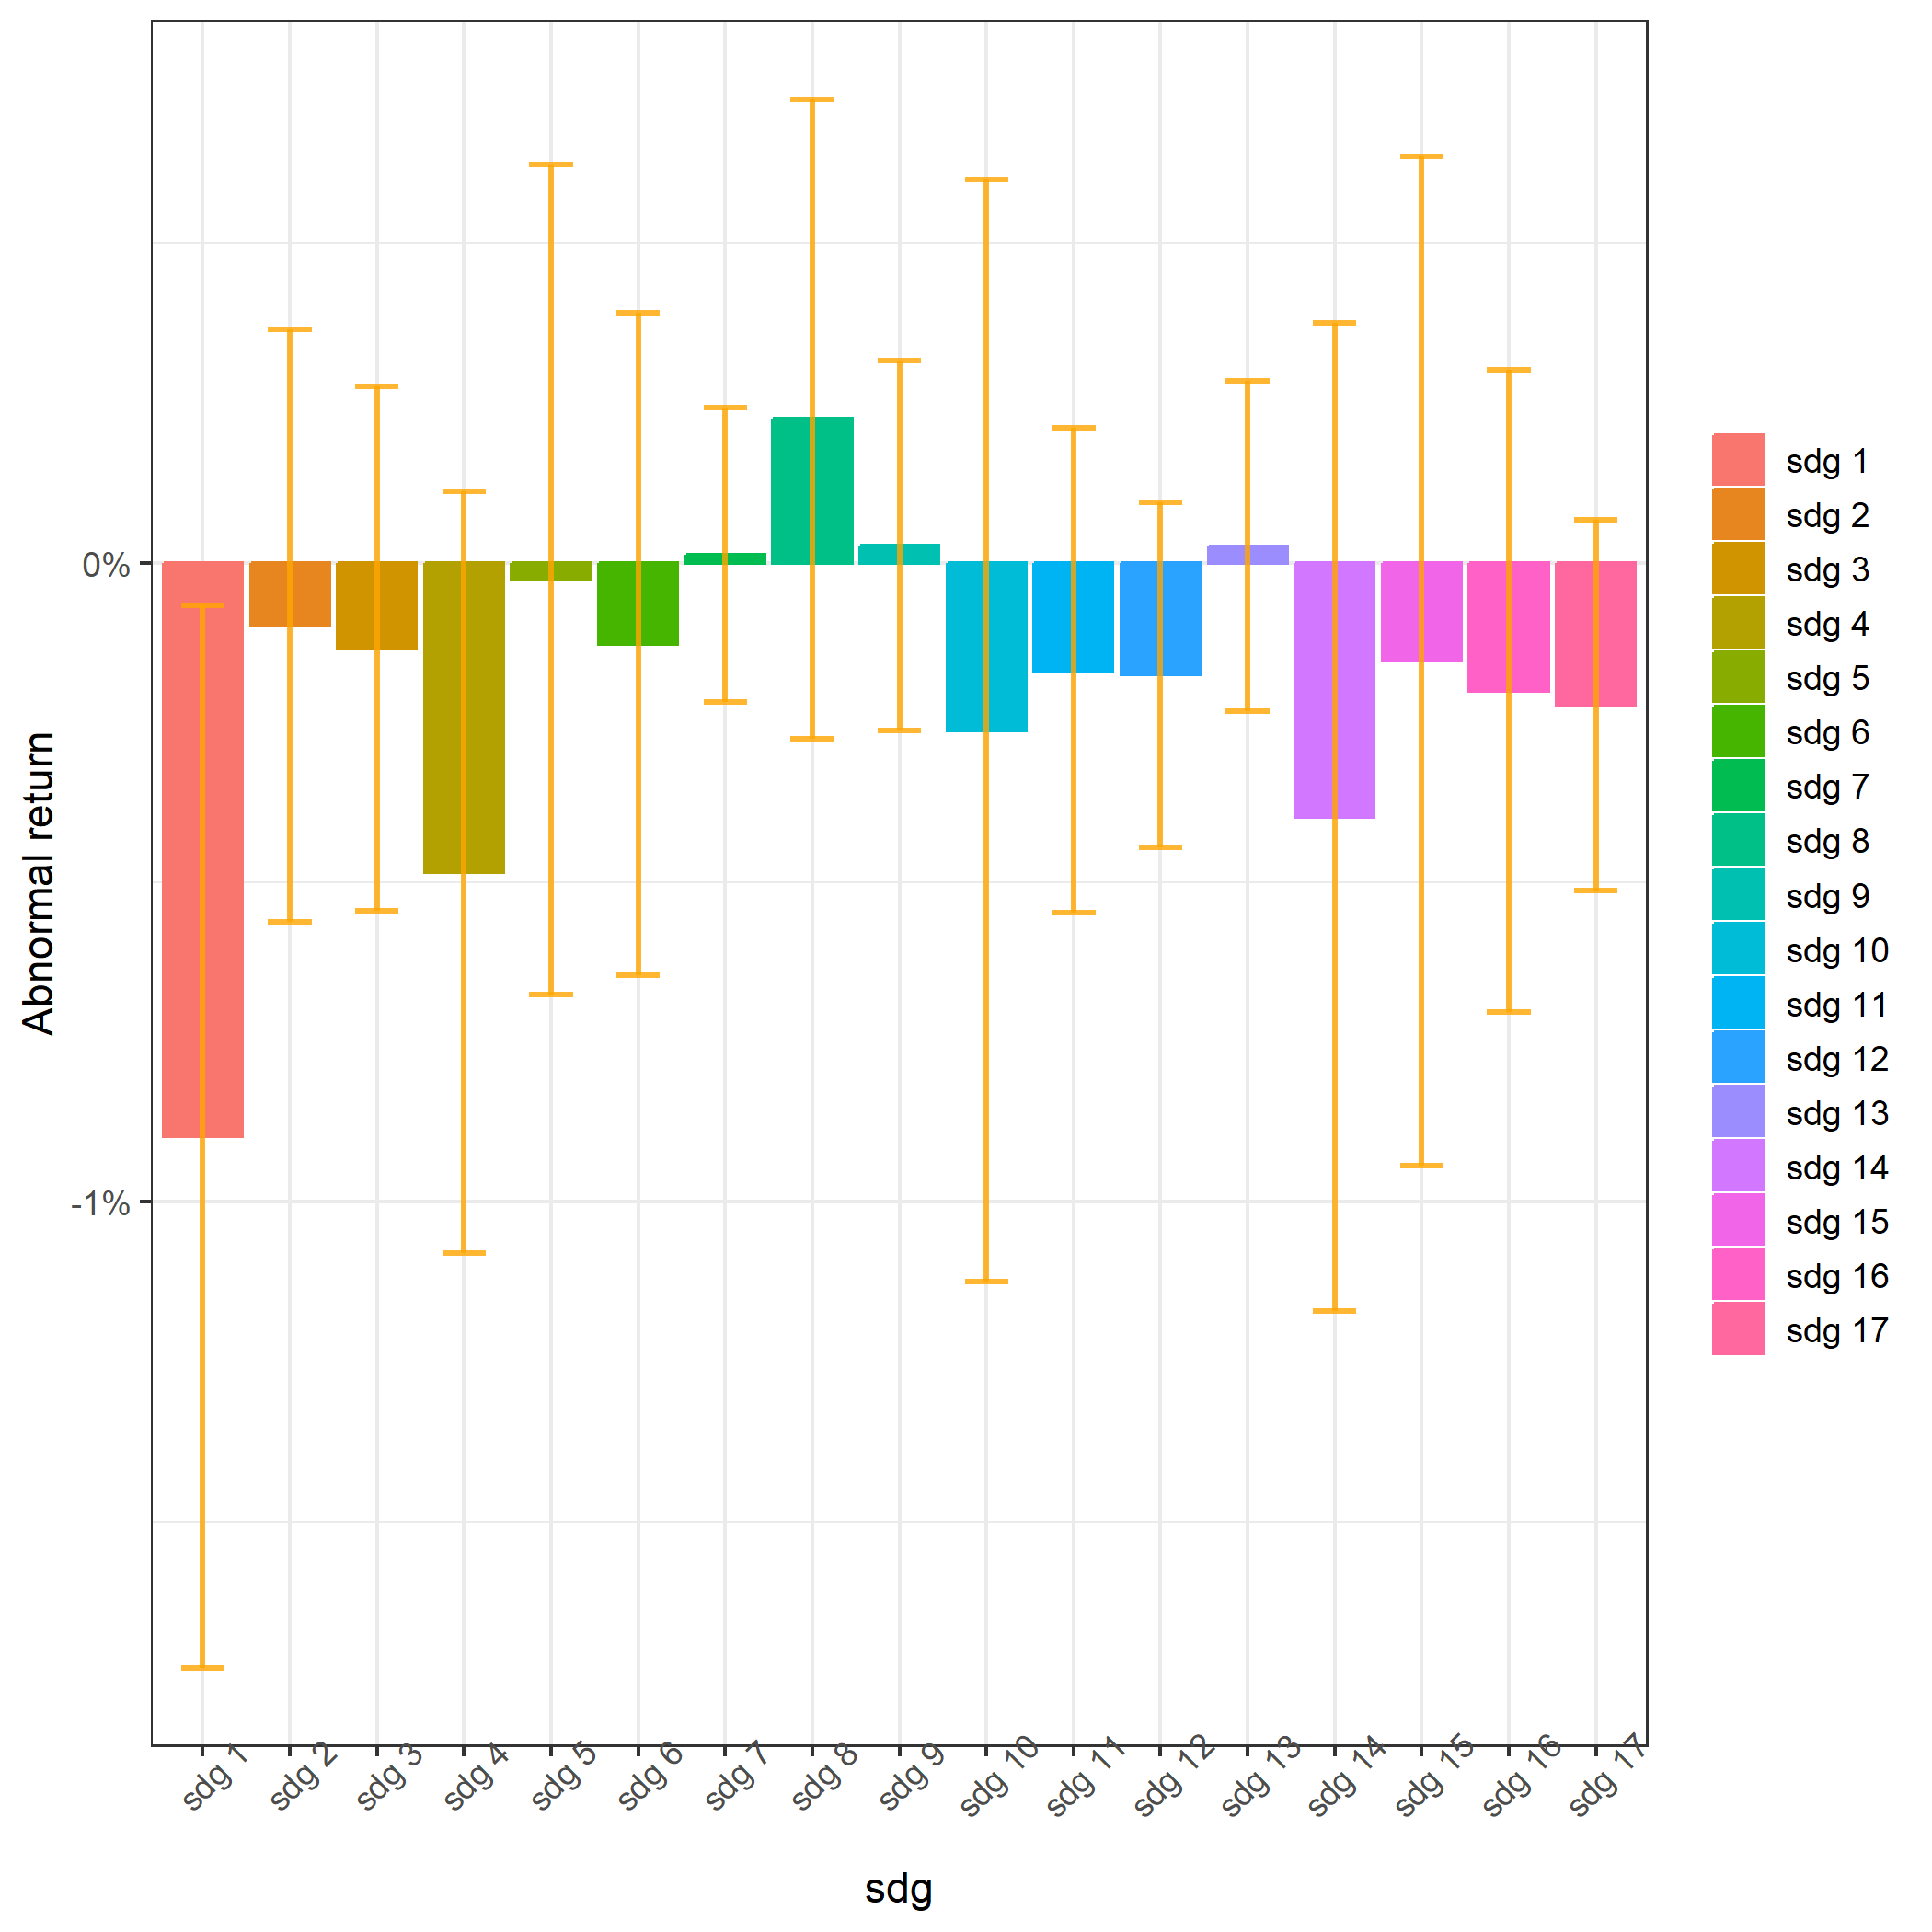
\includegraphics[scale=0.6]{Projekt/1.Figures analysis/ST_positive_sdg_bar.png}
    \caption*{\footnotesize The figure illustrates the AAR on $t = 0$ from positive news. The error bars represent the 95\% confidence intervals of the AAR.}
    \label{fig:ST_pos_bar}
\end{figure}


\noindent \textbf{Split firms on ESG rating.}
Splitting the sample firms by ESG risk ratings allows to investigate whether the investor reaction from positive news related to SDGs varies with the sustainability profile of the company. In the initial results from figure \ref{fig:ST_pos_news}, the CAAR were close to zero and estimated with large uncertainty. 

However, an average result like such doesn't report the full narrative as an evident difference between firms with a low and medium ESG risk profile is illustrated in figure  \ref{fig:ST_pos_ESG}. Allegedly, investors are pessimistic when low ESG risk-firms are involved in positive interactions with SDGs. The CAAR is significantly negative at $-0.5\%$ over the full window. Similarly, the high ESG risk-firms experience an average negative return, although the results are highly insignificant. The insignificance may be a feature of the low amount of observations relative to the other groups. In contrary, firms with a medium risk rating enjoy a significant, positive CAAR at $0.5\%$ over the full window. A clear distinction between the CAAR of low and medium risk profiles are already visible from around $t = -8$, where the two averages evolve conversely. 


\begin{figure} [H]
    \centering
    \caption{Positive news: CAAR split on ESG rating}
    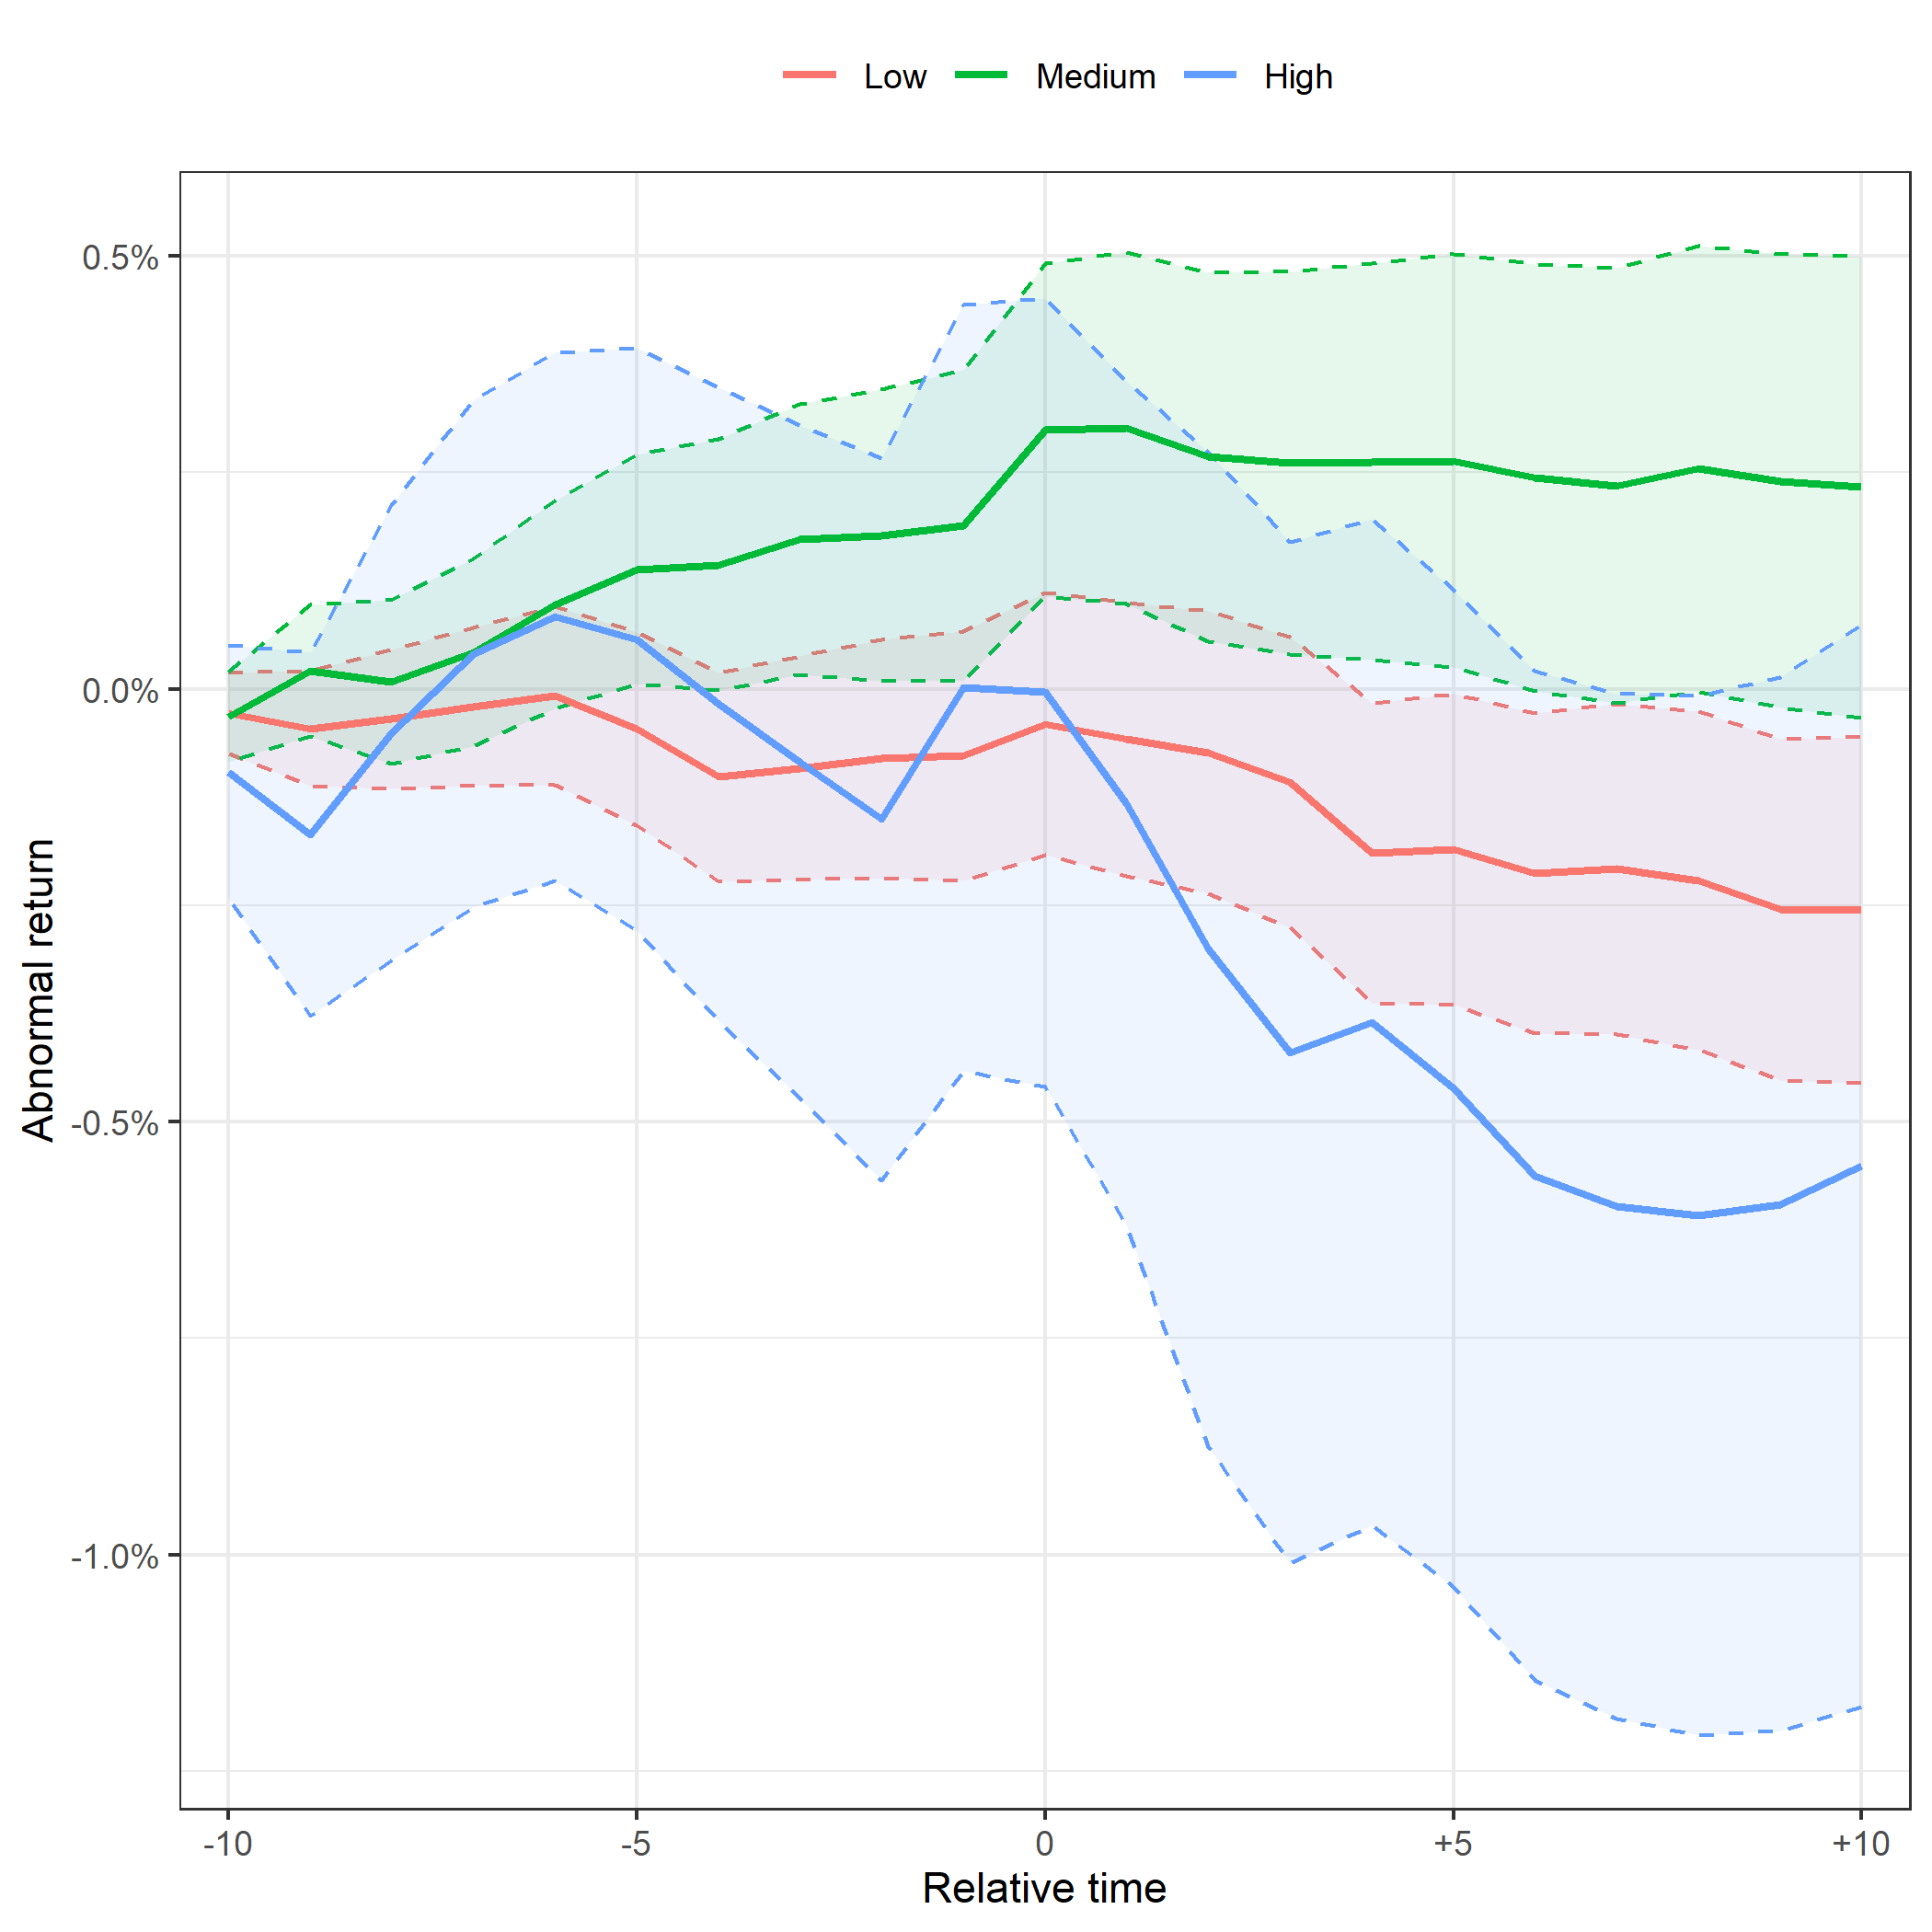
\includegraphics[scale=0.6]{Projekt/1.Figures analysis/ST_positive_ESG.png}
     \caption*{\footnotesize The figure illustrates the CAAR around the event date of positive news. The lines represent low, medium and high ESG risk of the firms in the sample. The ribbons represent the 95th confidence intervals. The categories low, medium, and high have, respectively, 1193, 1982, and 350 observed events in the sample.  }
    \label{fig:ST_pos_ESG}
\end{figure} 




Generally, the short term empirical evidence demonstrate a non-verifiable relation between positive events, related to both broad and specific SDGs, and abnormal returns. Positive news is however associated with an instant reaction from investors on the event date. The evidence point towards an overall negative relationship, but this is not statistically valid.  

% latex table generated in R 4.2.2 by xtable 1.8-4 package
% Mon Apr 17 10:17:44 2023
\begin{table}[H]
\centering
\begin{tabular}{cccccc}
  \hline
   & \multicolumn{2}{c}{Positive news} & \multicolumn{1}{p{1.5cm}}{} & \multicolumn{2}{c}{Negative news}  \\ \cline{2-3} \cline{5-6}
   \\
  Time & AAR & CAAR & & AAR & CAAR \\   
 \hline
-10 & -.0488 & -.0488 & & -.0547 & -.0547 \\ 
  -9 & -.0268 & -.0756 & & -.0217 & -.0764 \\ 
  -8 & .0281 & -.0475 & & .0198 & -.0566 \\ 
  -7 & .0225 & -.0249 & & .0143 & -.0423 \\ 
  -6 & .0445 & .0196 & & .0106 & -.0317 \\ 
  -5 & -.0022 & .0174 & & -.0679 & -.0996 \\ 
  -4 & .0385 & .0559 & & -.0916 & -.1912 \\ 
  -3 & .0329 & .0888 & &-.1448 & -.3361 \\ 
  -2 & -.0046 & .0843 & & -.1674 & -.5035 \\ 
  -1 & .0550 & .1393 & & -.2128 & -.7162 \\ 
  0 & .0819 & .2212 & &-.3781 & -1.0943 \\ 
  +1 & -.0356 & .1863 & & -.0462 & -1.1405 \\ 
  +2 & -.0654 & .1224 & & .0885 & -1.0520 \\ 
  +3 & -.0521 & .0714 & & .1399 & -.9175 \\ 
  +4 & .0068 & .0792 & & .0192 & -.8983 \\ 
  +5 & .0286 & .1074 & & .0068 & -.8916 \\ 
  +6 & -.0273 & .0804 & & .0457 & -.8449 \\ 
  +7 & -.0546 & .0268 & & -.0399 & -.8829 \\ 
  +8 & .0438 & .0709 & & .0164 & -.8665 \\ 
  +9 & .0118 & .0860 & & .0585 & -.8080 \\ 
  +10 & -.0114 & .0707 & & -.0085 & -.8223 \\ 
   \hline \hline
   \multicolumn{6}{p{10cm}}{\footnotesize Cumulative and simple average abnormal stock returns associated with positive and negative news over an event window of 21 days.} \\
   \hline
\end{tabular}
\caption{AAR and CAAR over event window (in percentage)} 
\end{table}



\subsection{Long term abnormal returns: The Calendar Time Portfolio} \label{sec: long_term_portfolio}

In contrast to the short term models, where the returns are measured relative to an event date, the long term portfolios are rebalanced each month and includes all firms, that have experienced an event within the T = 1/4/8/12 preceding months. The strategy resembles that T becomes the holding period for event firms. The portfolio returns are estimated over the full sample period of five years, and are evaluated by a regression on the market excess return and the factors from the Fama-French \citeyear{Fama_french_3fac} three-factor model. Full regression statistics including coefficient estimates, r-squared, and standard errors are available in Appendix X. The factor models do generally have high power in explaining the excess return risk exposure, with a r-square coefficient between 73\% to 98\% throughout the various portfolios. The portfolios which hold the least amount of firms on average generally has the lowest r-squared, which generally is a result of increased variance with less observations.  


\subsubsection{Negative news}

The abnormal returns from the individual portfolios are reflected through the regression intercept from the Fama-French model, presented as the Alpha in table \ref{tab: FF3-neg} along with the corresponding t-value. The table include the mean monthly number of firms in each portfolio as "N". Moreover, the conditional event specifications are partly disclosed as the 1, 2 and 3 "SD" gives the required number of standard deviations larger than the mean for an event to be identified as consequential and thus the firm selected to the portfolio. Above each horizontal line, the "$T = x$" express the portfolio holding period after an event has occurred. 

In the matter of negative events the alphas are negative for all portfolio specifications, which indicates a proper event selection methodology. However, the alphas are only significant in three instances. With a 1 SD requirement the alpha is significant for holding periods of $T = 1$ and $T = 4$ months at, respectively, -0.84\% at a $1\%$ level and -0.36\% at $5\%$. The portfolio with a 2 SD requirement and a $T=4$ holding period has significant alpha of -0.45\% at $5\%$. The alphas for holding periods larger than $T = 4$ are closer to zero and insignificant, which is in support of market efficiency over the long term. An implication of the strategy is that portfolios with longer holding periods will accordingly include more firms in each rebalancing, which ultimately will drive the portfolio return closer to the market return. For example with 1 SD, we see the inverse relation between the increases in the average N and the correspondingly decreases in alpha. In contrast, a higher SD requirement is equivalent to a more strict selection procedure designating that fewer firms will enter the portfolio. A consequence of the strict requirements is the size of the portfolios. A portfolio consisting of 5 or 10 firms will inevitably be exposed to idiosyncratic risks from the individual companies, which means that the portfolio outcome may be driven by specific risks rather than the effect from negative news. This effect is clear from the portfolio with $SD = 3$ and $T=1$, which generates an alpha of -0.78. As the alpha is relatively negative, one would expect that it would be significant as well, but the low amount of firms clearly brings too much variance into the model for the regression to be able to explain it. A large portfolio consisting of, e.g., 60 firms will not encounter the same risks due to diversification benefits. Diversification of random firms with monthly rebalancing is exactly the purpose of an exercise like this, since it allows to approximately isolate the effect of negative news from stock returns. 

\setlength{\tabcolsep}{15pt}
\begin{table}[h]
\small
\centering
\caption{Fama-French five-factor model alpha from negative news } 
\begin{tabular}{llllllc}
\hline \hline \\ 
 &     &  &    1 SD  &  2 SD  &  3 SD  &  \\    \cline{4-6} 
& & & \multicolumn{3}{c}{ T = 1} & \\ \cline{2-6}
& Alpha (\%)  &  & -0.84^{***}  & -0.47  & -0.78 &  \\ 
& t-value &  & -2.97 & -1.33  & -1.63 &  \\
&  N       &  &  19    & 10  & 5  & \\
& & & \multicolumn{3}{c}{ T = 4} & \\ \cline{2-6}
& Alpha (\%)  &  & -0.36^{**}  & -0.45^{**}  &  -0.27 & \\
& t-value &  & -2.23 & -2.12  & -1.04 & \\
&  N       &  & 60      & 35  & 18  & \\
& & & \multicolumn{3}{c}{ T = 8} & \\ \cline{2-6}
& Alpha (\%)   &  & -0.15   & -0.14  & -0.12 &  \\
& t-value &  & -1.21  & -0.89 & -0.68 &  \\
& N       &  & 100 & 63   & 34 & \\
& & & \multicolumn{3}{c}{ T = 12} & \\ \cline{2-6}
& Alpha (\%)   &  & -0.08  & -0.16  & -0.17 &  \\
& t-value &  & -0.86  & -1.16 & -0.97 & \\
& N       &  & 130    & 86  & 48 \\ \hline \hline
 \multicolumn{7}{l}{ \footnotesize $^* \; p\; <\; 0.1$, $ ^{**} \; p\; <\; 0.05$, $ ^{***} \; p\; <\; 0.01$  } \\
 \multicolumn{7}{p{11.5cm}}{ \footnotesize Alpha is the WLS-regression intercept (in \%) of the Fama-French 3-factor model, displayed along with the corresponding t-value. N is the average amount of firms included in the portfolio each month, and T is the portfolio holding period. The threshold for event firms to be included in the portfolio is either 1,2 or 3 "SD" (standard deviations) larger than the mean.} \\ 
 \hline
\end{tabular}
\label{tab: FF3-neg}
\end{table}

Overall, the relation between negative news and returns are most severe within 1-4 months after an event has occurred and with a "loose" selection criteria of 1 SD for event firms to be included in the portfolio. Although most of the alphas are insignificant it is important to note that all are negative, which support the relation between negative news and pessimistic investor behavior.  
??. 


\subsubsection{Positive news}

The impact from positive news on financial performance in the long run is illustrated in table \ref{tab: FF3-pos}. The table applies the same format as table \ref{tab: FF3-neg}. Positive events have no significant impact on returns over any of the portfolio and event constructions. Nevertheless, the long run effect is predominantly negative, which appears in contrast to the short term effect, that indicate a positive relation, however insignificant. The performance is most negative when applying a brief holding period of $T=1$ and a strict event rule of $SD = 3$, which generates alpha of -0.42\%. With $T=1$ and $SD=1$ the portfolio achieves an alpha of -0.3\%.  
Such results are indicative of a pessimistic short-to-medium term investor reaction to general positive news. However, as the alphas are insignificant in all instances, the general conclusion is that there is no relation between positive news and stock returns. 

Applying holding periods longer than $T=1$ generates exclusively alphas close to zero, which resembles a well-diversified portfolio return close to the market portfolio, which is an expected result if positive news are recognized as irrelevant. 



\setlength{\tabcolsep}{15pt}
\begin{table}[]
\small
\centering
\caption{Fama-French five-factor model alpha from positive news } 
\begin{tabular}{ccccccc}
\hline \hline \\ 
 &     &  &    1 SD  &  2 SD  &  3 SD  &  \\ \cline{4-6} 
& & & \multicolumn{3}{c}{ T = 1} & \\ \cline{2-6}
& Alpha (\%)  &  & -0.26  & 0.04  & -0.37 &  \\
& t-value &  & -1.03 & 0.11  & -0.74 & \\
&  N       &  &  34    & 15 & 7 &\\
& & & \multicolumn{3}{c}{ T = 4} & \\ \cline{2-6}
& Alpha (\%)  &  & -0.04  & 0.03  &  -0.07 & \\
& t-value &  & -0.26 & 0.13  & -0.23 & \\
& N       &  & 105     & 52  & 25 & \\
& & & \multicolumn{3}{c}{ T = 8} & \\ \cline{2-6}
& Alpha (\%)  &  & 0.01   & -0.01  & 0.04 &  \\
& t-value &  & 0.05  & -0.15 & 0.18 & \\
& N       &  & 164 & 63   & 47 & \\
&  & & \multicolumn{3}{c}{ T = 12} & \\ \cline{2-6}
& Alpha (\%)  &  & 0.05  & 0.13  & 0.23 &  \\
& t-value &  & 0.76  & 1.09 & 1.35 & \\
& N       &  & 202   & 122  & 67 & \\ \hline \hline
 \multicolumn{7}{l}{ \footnotesize $^* \; p\; <\; 0.1$, $ ^{**} \; p\; <\; 0.05$, $ ^{***} \; p\; <\; 0.01$  } \\
 \multicolumn{7}{p{11.5cm}}{ \footnotesize Alpha is the WLS-regression intercept (in \%) of the Fama-French 3-factor model, displayed along with the corresponding t-value. N is the average amount of firms included in the portfolio each month, and T is the portfolio holding period. The threshold for event firms to be included in the portfolio is either 1,2 or 3 "SD" (standard deviations) larger than the mean.}  \\ 
\end{tabular}
\label{tab: FF3-pos}
\end{table}

